\section{Interchanging and Stacking VOL Plugins}
Accessing an HDF5 container with a VOL plugin different than the one
it was created with would be a valid approach as long as the
underlying file format is the same. This would be the user’s
responsibility to ensure that the different plugins are
interchangeable.

\subsection{Stacking Plugins on Top of Each Other}
It would be also possible to stack VOL plugins on top of each
other. This notion is similar to the idea of the split VFD, where
underneath the split VFD itself, two file drivers would be used, one
for the file storing the metadata and another for raw data. Some
stackings make sense and others would be erroneous. For example,
stacking the native HDF5 plugin on top of a non-HDF5 backend plugin
does not make sense and is erroneous. Figure~\ref{stack} shows a
stacking of a remote plugin, where data is distributed remotely, on
top of the native h5 plugin, where servers that store the data at
remote locations use the h5 file format.

\begin{figure}[ht!]
\centering
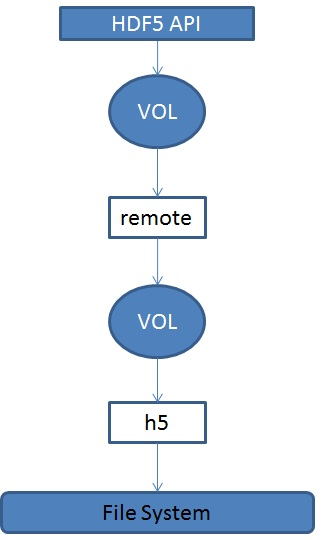
\includegraphics[width=90mm]{stacked.jpg}
\caption{Stacked VOL plugins.}
\label{stack}
\end{figure}

\subsection{Mirroring Plugins}
Another useful design option is to allow a mirroring plugin, where the
HDF5 API calls are forwarded through a mirror plugin to two or more
VOL plugins. This is an extention to the stacking
feature. Figure~\ref{mirror} shows an example of a VOL mirror that
maps HDF5 API calls to an h5 backend plugin and an XML backend plugin.

\begin{figure}[ht!]
\centering
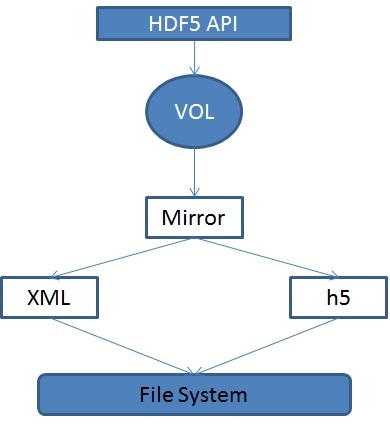
\includegraphics[width=90mm]{mirrored.jpg}
\caption{Mirrored VOL plugins.}
\label{mirror}
\end{figure}

Another possible VOL plugin could be a statistics plugin that just
gathers information on HDF5 API calls and records statistics
associated with the number of calls to a specific API functions and
corresponding parameters. This plugin would be very useful for
profiling purposes. The statistics plugin would be stacked on top of
another VOL plugin that actually performs the required access to the
file.

\subsection{Implementing Stacked and Mirrored Plugins}
A new set of API calls that map directly to the VOL callbacks have
been added to the HDF5 library to make stacking and mirroring easy for
plugin developers. Similarly to the public VFD (H5FD) routines that
call the VFD callbacks directly, we added the following H5VL APIs to
the library:

\begin{lstlisting}
/* ATTRIBUTE OBJECT ROUTINES */
void *H5VLattr_create(void *obj, H5VL_loc_params_t loc_params, H5VL_t *vol_plugin, const char *attr_name, hid_t acpl_id, hid_t aapl_id, hid_t dxpl_id, void **req);
void *H5VLattr_open(void *obj, H5VL_loc_params_t loc_params, H5VL_t *vol_plugin, const char *name, hid_t aapl_id, hid_t dxpl_id, void **req);
herr_t H5VLattr_read(void *attr, H5VL_t *vol_plugin, hid_t dtype_id, void *buf, hid_t dxpl_id, void **req);
herr_t H5VLattr_write(void *attr, H5VL_t *vol_plugin, hid_t dtype_id, const void *buf, hid_t dxpl_id, void **req);
herr_t H5VLattr_iterate(void *obj, H5VL_loc_params_t loc_params,
H5VL_t *vol_plugin, H5_index_t idx_type, H5_iter_order_t order,
hsize_t *n, H5A_operator2_t op, void *op_data, hid_t dxpl_id, void **req);
herr_t H5VLattr_get(void *attr, H5VL_t *vol_plugin, H5VL_attr_get_t get_type, hid_t dxpl_id, void **req, va_list arguments);
herr_t H5VLattr_remove(void *obj, H5VL_loc_params_t loc_params, H5VL_t
*vol_plugin, const char *attr_name, hid_t dxpl_id, void **req);
herr_t H5VLattr_close(void *attr, H5VL_t *vol_plugin, hid_t dxpl_id, void **req);

/* DATASE OBJECT ROUTINES */
void *H5VLdataset_create(void *obj, H5VL_loc_params_t loc_params,
H5VL_t *vol_plugin, const char *name, hid_t dcpl_id, hid_t dapl_id, hid_t dxpl_id, void **req);
void *H5VLdataset_open(void *obj, H5VL_loc_params_t loc_params, H5VL_t
*vol_plugin, const char *name, hid_t dapl_id, hid_t dxpl_id, void **req);
herr_t H5VLdataset_read(void *dset, H5VL_t *vol_plugin, hid_t
mem_type_id, hid_t mem_space_id, hid_t file_space_id, hid_t plist_id, void *buf, void **req);
herr_t H5VLdataset_write(void *dset, H5VL_t *vol_plugin, hid_t
mem_type_id, hid_t mem_space_id, hid_t file_space_id, hid_t plist_id, const void *buf, void **req);
herr_t H5VLdataset_set_extent(void *dset, H5VL_t *vol_plugin, const hsize_t size[], hid_t dxpl_id, void **req);
herr_t H5VLdataset_get(void *dset, H5VL_t *vol_plugin,
H5VL_dataset_get_t get_type, hid_t dxpl_id, void **req, va_list arguments);
herr_t H5VLdataset_close(void *dset, H5VL_t *vol_plugin, hid_t dxpl_id, void **req);

/* DATATYPE OBJECT ROUTINES */
void *H5VLdatatype_commit(void *obj, H5VL_loc_params_t loc_params, H5VL_t *vol_plugin, const char *name, hid_t type_id, hid_t lcpl_id, hid_t tcpl_id, hid_t tapl_id, hid_t dxpl_id, void **req);
void *H5VLdatatype_open(void *obj, H5VL_loc_params_t loc_params, H5VL_t *vol_plugin, const char *name, hid_t tapl_id, hid_t dxpl_id, void **req);
ssize_t H5VLdatatype_get_binary(void *obj, H5VL_t *vol_plugin, unsigned char *buf, size_t size, hid_t dxpl_id, void **req);
herr_t H5VLdatatype_get(void *obj, H5VL_t *vol_plugin, H5VL_datatype_get_t get_type, hid_t dxpl_id, void **req, va_list arguments);
herr_t H5VLdatatype_close(void *dt, H5VL_t *vol_plugin, hid_t dxpl_id,
void **req);

/* FILE OBJECT ROUTINES */
void *H5VLfile_create(H5VL_t **vol_plugin, const char *name, unsigned flags, hid_t fcpl_id, hid_t fapl_id, hid_t dxpl_id, void **req);
void *H5VLfile_open(H5VL_t **vol_plugin, const char *name, unsigned flags, hid_t fapl_id, hid_t dxpl_id, void **req);
herr_t H5VLfile_flush(void *obj, H5VL_loc_params_t loc_params, H5VL_t *vol_plugin, H5F_scope_t scope, hid_t dxpl_id, void **req);
herr_t H5VLfile_misc(void *file, H5VL_t *vol_plugin, H5VL_file_misc_t misc_type, hid_t dxpl_id, void **req, va_list arguments);
herr_t H5VLfile_optional(void *file, H5VL_t *vol_plugin,
H5VL_file_optional_t optional_type, hid_t dxpl_id, void **req, va_list arguments);
herr_t H5VLfile_get(void *file, H5VL_t *vol_plugin, H5VL_file_get_t get_type, hid_t dxpl_id, void **req, va_list arguments);
herr_t H5VLfile_close(void *file, H5VL_t *vol_plugin, hid_t dxpl_id, void **req);

/* GROUP OBJECT ROUTINES */
void *H5VLgroup_create(void *obj, H5VL_loc_params_t loc_params, H5VL_t
*vol_plugin, const char *name, hid_t gcpl_id, hid_t gapl_id, hid_t dxpl_id, void **req);
void *H5VLgroup_open(void *obj, H5VL_loc_params_t loc_params, H5VL_t
*vol_plugin, const char *name, hid_t gapl_id, hid_t dxpl_id, void
**req);
herr_t H5VLgroup_get(void *obj, H5VL_t *vol_plugin, H5VL_group_get_t get_type, hid_t dxpl_id, void **req, va_list arguments);
herr_t H5VLgroup_close(void *grp, H5VL_t *vol_plugin, hid_t dxpl_id, void **req);

/* LINK OBJECT ROUTINES */
herr_t H5VLlink_create(H5VL_link_create_type_t create_type, void *obj,
H5VL_loc_params_t loc_params, H5VL_t *vol_plugin, hid_t lcpl_id, hid_t
lapl_id, hid_t dxpl_id, void **req);
herr_t H5VLlink_move(void *src_obj, H5VL_loc_params_t loc_params1,
void *dst_obj, H5VL_loc_params_t loc_params2, H5VL_t *vol_plugin,
hbool_t copy_flag, hid_t lcpl_id, hid_t lapl_id, hid_t dxpl_id, void **req);
herr_t H5VLlink_iterate(void *obj, H5VL_loc_params_t loc_params,
H5VL_t *vol_plugin, hbool_t recursive, H5_index_t idx_type,
H5_iter_order_t order, hsize_t *idx, H5L_iterate_t op, void *op_data, hid_t dxpl_id, void **req);
herr_t H5VLlink_get(void *obj, H5VL_loc_params_t loc_params, H5VL_t
*vol_plugin, H5VL_link_get_t get_type, hid_t dxpl_id, void **req, va_list arguments);
herr_t H5VLlink_remove(void *obj, H5VL_loc_params_t loc_params, H5VL_t
*vol_plugin, hid_t dxpl_id, void **req);

/* OBJECT ROUTINES */
void *H5VLobject_open(void *obj, H5VL_loc_params_t loc_params, H5VL_t *vol_plugin, H5I_type_t *opened_type, hid_t dxpl_id, void **req);
herr_t H5VLobject_copy(void *src_obj, H5VL_loc_params_t loc_params1,
H5VL_t *vol_plugin1, const char *src_name, void *dst_obj,
H5VL_loc_params_t loc_params2, H5VL_t *vol_plugin2, const char *dst_name, hid_t ocpypl_id, hid_t lcpl_id, hid_t dxpl_id, void **req);
herr_t H5VLobject_visit(void *obj, H5VL_loc_params_t loc_params,
H5VL_t *vol_plugin, H5_index_t idx_type, H5_iter_order_t order, H5O_iterate_t op, void *op_data, hid_t dxpl_id, void **req);
herr_t H5VLobject_get(void *obj, H5VL_loc_params_t loc_params, H5VL_t
*vol_plugin, H5VL_object_get_t get_type, hid_t dxpl_id, void **req, va_list arguments);
herr_t H5VLobject_misc(void *obj, H5VL_loc_params_t loc_params, H5VL_t
*vol_plugin, H5VL_object_misc_t misc_type, hid_t dxpl_id, void **req, va_list arguments);
herr_t H5VLobject_optional(void *obj, H5VL_loc_params_t loc_params,
H5VL_t *vol_plugin, H5VL_object_misc_t optional_type, hid_t dxpl_id, void **req, va_list arguments);
herr_t H5VLobject_close(void *obj, H5VL_loc_params_t loc_params, H5VL_t *vol_plugin, hid_t dxpl_id, void **req);

/* ASYNCHRONOUS ROUTINES */
herr_t H5VLrequest_cancel(void **req, H5VL_t *vol_plugin, H5ES_status_t *status);
herr_t H5VLrequest_test(void **req, H5VL_t *vol_plugin, H5ES_status_t *status);
herr_t H5VLrequest_wait(void **req, H5VL_t *vol_plugin, H5ES_status_t *status);
\end{lstlisting}

The above API calls should be used in the stacked or mirror plugin to
call into the lower plugins indicated by the {\tt vol\_plugin}
parameter that is added to all the routines.

%%% Local Variables: 
%%% mode: latex
%%% TeX-master: t
%%% End: 
